\section{Home Assistant}
\label{sec:homeassistant}
    Eine der etablierten \acl{SH} Plattformen ist das sogenannte Home Assistant System. Die Open-Source-Software ist ein zentrales 
    Steuerungssystem von Heimautomationen, ebenso ist eine Verwaltung von intelligenten Geräten mit dem Fokus der lokalen Steuerung und Sicherung der 
    Privatsphäre möglich. Der Zugriff kann über die Smartphone-App, jeweils verfügbar für iOS und Android, oder über die webbasierte 
    Benutzeroberfläche (Web-App) erfolgen. In dem lokalen System können Geräte per Sprachbefehl gesteuert werden. Kompatible 
    Plattformen sind unter anderem Google Assistant, Amazon Alexa und Apple HomeKit. %Dies sind weitaus nur eine Selektion von bekannten 
    %Herstellern. 
    Home Assistant bietet eine vielfältigere Verknüpfung von Geräten, Services und Plattformen. Die zentrale Steuerung 
    unterstützt durch modulare Integrationskomponenten die einzelnen Geräte, Anwendungen und Services. Für die drahtlose Kommunikation 
    werden native Integrationskomponenten verwendet, darunter Bluetooth, ZigBee und Z-Wave. Diese werden verwendet, um lokale \ac{PAN} mit 
    Geräten mit geringem Stromverbrauch aufzubauen. Die Steuerung kann mit proprietären Ökosystemen stattfinden, sofern diese eine offene 
    \acs{API} oder Anbindungen über \acs{MQTT} anbieten.\footnote{Definition von Home Assistant. \url{https://en.wikipedia.org/wiki/Home_Assistant} Besucht am 16.04.2022}
    \\
    Die Platform ist in Python geschrieben, wird aktiv instand gehalten und durch eine große Community unterstützt. Die Software ist allgemein unter 
    der Apache 2.0, veröffentlicht. Der folgende Abschnitt befasst sich in Kürze mit der Historie des Systems. 
    
    \subsection*{Historie}
    \label{sec:historyHOAS}
        Anfang des vierten Quartals im Jahr 2013 startete das Python-Projekt von Paulus Schoutsen und wurde im November 2013 erstmals auf GitHub 
        veröffentlicht.\footnote{Anfänge von Home Assistant. \url{https://www.linux.com/topic/embedded-iot/home-assistant-python-approach-home-automation/} Besucht am 18.04.2022}
        \\
        \linebreak
        Vier Jahre nach den ersten Entwicklungen der \acl{SH} Plattform wurde im Juli 2017 ein verwaltetes Betriebssystem mit dem Namen 
        \textit{Hass.io} implementiert.\footnote{Verkündungen von Home Assistant. \url{https://www.home-assistant.io/blog/categories/announcements/} Besucht am 18.04.2022} 
        Dadurch gelang der Durchbruch der vereinfachten Verwendung der Home Assistant Plattform auf kleineren Computern, sogenannten 
        Einplatinencomputern, wie beispielsweise ein Gerät der Raspberry Pi Serie. In Zusammenhang mit dem Betriebssystem kam ein 
        \textit{Supervisor}-Verwaltungssystem hinzu, das den Benutzern die Verwaltung, Sicherung und Aktualisierung der lokalen Installation 
        erleichtert. Ein weiteres Feature des Supervisors ist die Möglichkeit, der Plattform über Add-ons weitere Funktionalitäten zur Verfügung zu 
        stellen.\footnote{Einstieg in das Hass.io Betriebssystem. \url{https://www.home-assistant.io/blog/2017/07/25/introducing-hassio/} Besucht am 18.04.2022}
        \\
        \linebreak
        Die Software wird stetig weiterentwickelt und verbessert. Mittlerweile gehört sie zu den am meisten genutzten Open-Source-Plattformen 
        im Bereich \acl{SH}.

\subsection{Konzept und Architektur}
\label{sec:conceptArchitectureHAOS}
    Home Assistant bietet eine Plattform für die zentrale Haussteuerung und die damit einhergehende Steuerung von Heimautomationen. Die 
    Software ist nicht nur eine einfache Steuerungs- und Konfigurationssoftware, sondern ein eingebettetes Betriebssystem, das 
    verbraucher- und nutzerorientiert das Verwenden und Konfigurieren von Haussteuerungen erleichtert. \footnote{Konzept und Architektur von Home Assistant. \url{https://developers.home-assistant.io/docs/architecture_index} Besucht am 19.04.2022}
    \\
    \linebreak
    Damit der offene Ansatz von Home Assistant gegenüber Anbietern von intelligenten Geräten nicht eingeschränkt ist, bietet die Software Möglichkeiten, um viele 
    Geräte zu integrieren und über die Plattform zu nutzen. Somit begegnet Home Assistant der Heterogenität des offenen Marktes, in sofern, dass diese Geräte auf  
    gemeinsame Konzepte gebracht werden. Diese sind in vier Konzepte %\footnote{Erläuterung der Konzepte von Home Assistant. \url{https://apiumhub.com/tech-blog-barcelona/domotics-with-home-assistant-concepts/} Besucht am 21.04.2022} 
    aufgeteilt, mit der die Vereinheitlichung vorangetrieben werden kann: 
    \begin{itemize}
        \item Integration (Integration): Integrationen repräsentieren die Geräte und Dienste innerhalb der Home Assistant Anwendung. 
              Ebenso können mittels Integrationen Daten von Datenpunkten abgerufen werden.
        \item Gerät (Device): Nach der Konfiguration der Integration werden die Geräte in Home Assistant angelegt. 
              Diese werden dann als erkannte Geräte der Integration dargestellt, z.B. als Temperatur-, Licht- oder Feuchtigkeitssensor.
        \item Entität (Entity): Die Datenpunkte sind die Geräte, die sogenannten Entitäten, die durch die Integrationen standardisiert werden. 
              Dies sind Objekte, die Funktionalitäten oder Daten des Gerätes darstellen, z.B. die Temperatur, Helligkeit oder die Feuchtigkeit.
        \item Automatisierung (Automation): Automatisierungen sind Prozesse, die bei einem bestimmten ausgelösten Event ausgeführt werden 
              sollen. Diese Auslöser (Trigger) können Zeitpunkte, Ereignisse oder manuell gesteuerte Aktionen des Nutzers sein, z.B. das 
              Ausschalten des Bürolichts, wenn durch einen Bewegungssensor fünf Minuten keine Bewegung festgestellt wurde oder wenn der 
              Helligkeitswert, der über den Sensor festgestellt wurde, einen bestimmten Wert erreicht hat, soll das Licht ebenso 
              ausgeschaltet werden.
    \end{itemize}
    Die Architektur der Home Assistant Anwendung ist grundlegend als eingebettetes System eines Betriebssystems aufgestellt, welches in 
    drei Schichten aufgeteilt ist. In unterster Ebene befindet sich das Betriebssystem, welches als minimales Linux System postiert 
    ist, um die darauf liegenden Schichten, den Aufseher (Supervisor) und den Kern (Core), zu betreiben. Mit dem Supervisor wird das 
    Betriebssystem verwaltet und konfiguriert. Der eigentliche Kern interagiert mit dem Supervisor, den Geräten und den Services. 
    \\
    \linebreak
    Der Supervisor ist die Schicht über dem Betriebssystem. Die Kommunikation der beiden Komponenten findet über einen D-Bus statt. Diese Zwischenschicht ermöglicht dem 
    Benutzer die Verwaltung der Home Assistant Installation. 
    \\
    Die Aufgaben des Supervisors sind wie folgt 
    definiert\footnote{Architektur des Supervisors. \url{https://developers.home-assistant.io/docs/supervisor} Besucht am 22.04.2022}. 
    \begin{itemize}
        \item Dieser führt den Home Assistant Kern (Core) aus.
        \item Dieser führt die Updates des Home Assistant Core aus.
        \item Dieser führt einen \textit{Rollback} bei fehlgeschlagenem Update durch.
        \item Dieser führt Sicherungen und Wiederherstellungen durch.
        \item Dieser verwaltet die Add-ons der Core Instanz.
    \end{itemize}
    \begin{figure}[hbt!]
        \centering
        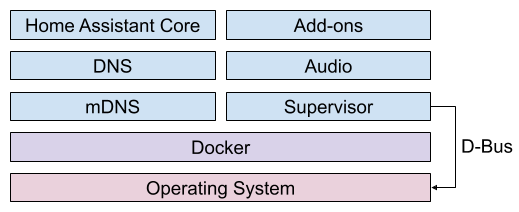
\includegraphics[width=10cm,height=10cm,keepaspectratio]{images/ha_architecture_2020.png}
        \caption{Architektur des Home Assistant Supervisors \cite{haos-supervisor}}
        \label{fig:architectureHAOS}
    \end{figure}
    Die auf dem Supervisor aufbauende Architektur ist die der Anwendung, der sogenannte Core. Dieser besteht aus vier 
    Komponenten, welche den Hauptteil abbilden: Event Bus, State Machine, Service Registry und Timer\footnote{Entwickler Dokumentation der Plattform. \url{https://developers.home-assistant.io/docs/} Besucht am 24.04.2022}. 
    \\
    Mit dem Event Bus wird das Abhören und Auslösen von Events und Ereignisse erleichtert. Die Komponente stellt eine Eigenschaft 
    der Home Assistant Anwendung dar. Die Zustandsmaschine (State Machine) ist eine weitere Komponente, mit der die Zustände der Gegenstände, wie  
    Sensoren, Service- oder Saugroboter uvm., überwacht und deren Änderungsereignisse an den Event Bus ausgelöst werden. 
    Mit der Dienstregistrierung (Service Registry) wird der Event Bus auf eingehende Aufrufe von 
    Diensten abgehört. Über die Service Registry kann der Benutzer Dienste hinzufügen und verwalten. Mittels der Entwicklertools, die über das 
    \ac{UI} aufgerufen werden können, kann der Benutzer die Dienste und Automatisierungen anwählen und konfigurieren. Das letzte 
    Element, der Timer, ist ebenso eine Komponente der Architektur, die zeitveränderte Ereignisse gemäß einer gegebenen Frequenz 
    an den Event Bus sendet. Somit können zeitbasierte Automatisierungen vereinfacht und ausgelöst werden. Als Datenbank wird eine 
    nicht cloudbasierte SQLite\footnote{Structured Query Language, eine Datenbanksprache zur Definition, Abfrage und Bearbeitung von Datenstrukturen in relationalen Datenbanken} 
    Datenbank verwendet. Diese ist nur auf dem Gerät enthalten und wird nicht über das Internet übertragen. 
    Im lokalen Netzwerk hat der Nutzer die Möglichkeit, auf die Datenbank zuzugreifen und eine Historie von Aktionen einzusehen. 
    Eine Verlaufskomponente, die ebenso im Core enthalten ist, speichert die Ereignisse innerhalb der Plattform. Somit können Nutzer auf 
    alle gespeicherten Informationen zu Hause zugreifen und diese einsehen \cite{HAOSarchitecture2018}.
    \\
    \linebreak
    \begin{figure}[hbt!]
        \centering
        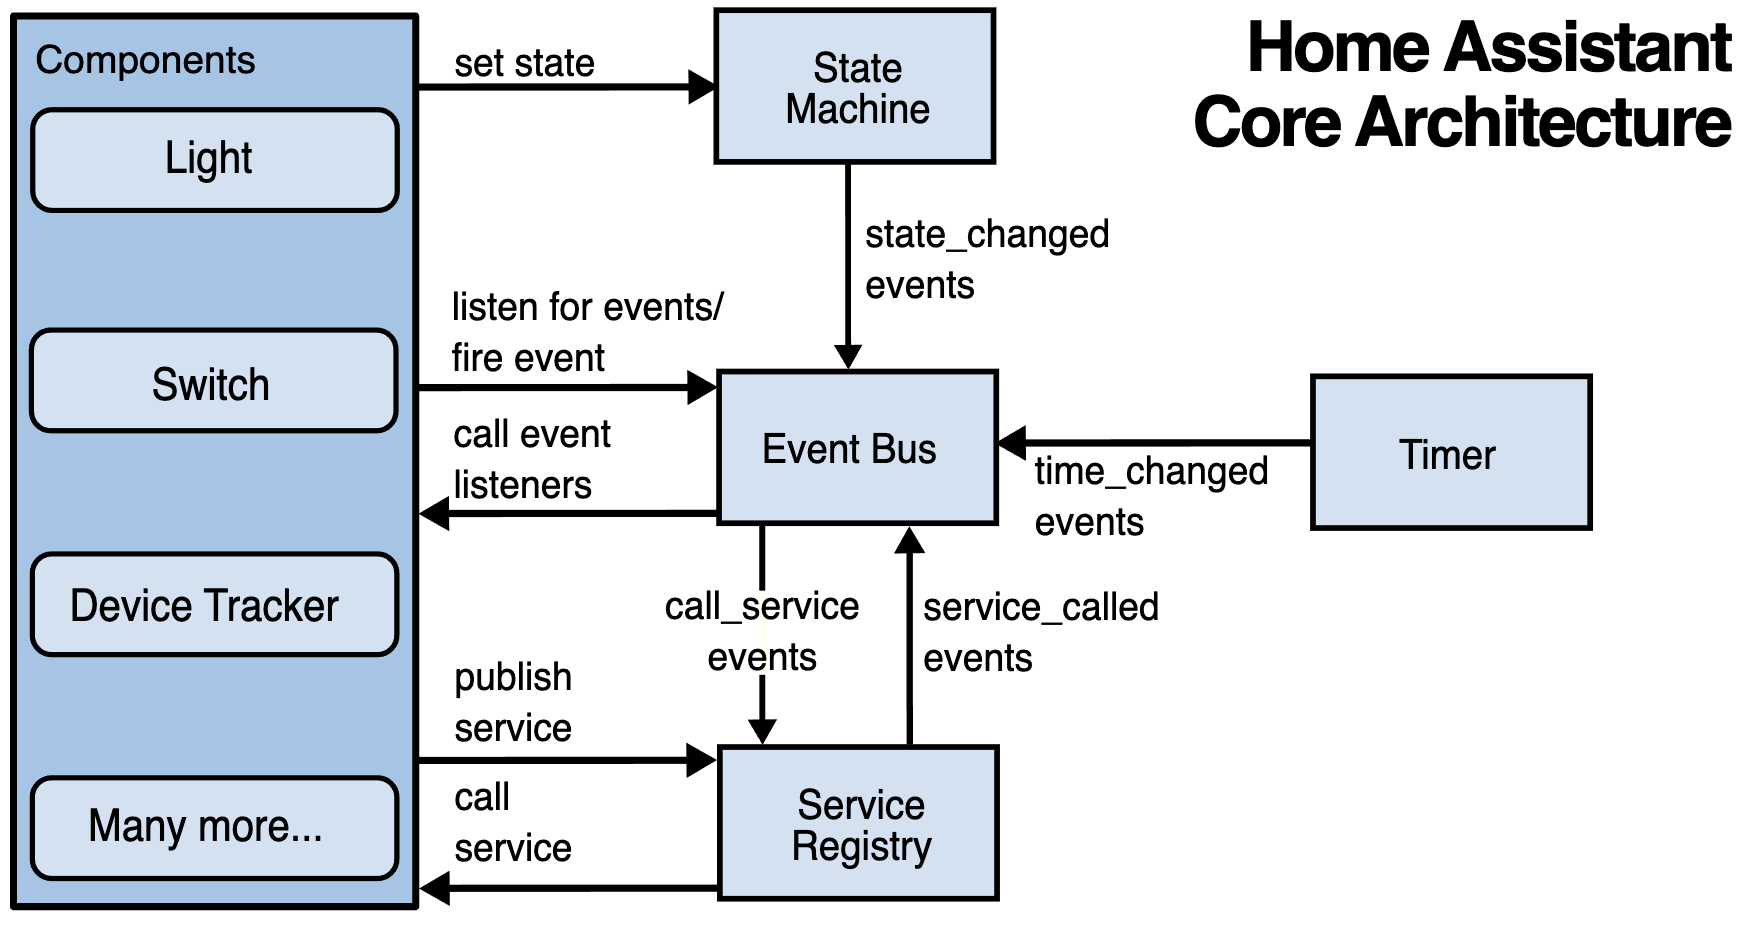
\includegraphics[width=15cm,height=15cm,keepaspectratio]{images/HAOS_Core_Architecture.png}
        \caption{Architektur des Home Assistant Cores \cite{HAOSarchitecture2018}}
        \label{fig:architectureHAOSCore}
    \end{figure}
\subsection{Ziele und Schwerpunkte}
    Jede Softwarelösung verfolgt bestimmte Ziele und Schwerpunkte, um die Zielerreichung, die sog. \ac{DOD}, messbar zu machen. Die mit 
    der Home Assistant Plattform verfolgten Ziele sind unter anderem der Schutz der Privatsphäre und die Datensicherheit, die Wahlmöglichkeit zur Anbindung von 
    Geräten und die Haltbarkeit der Plattform\footnote{Schwerpunkte der Home Assistant Plattform. \url{https://www.home-assistant.io/blog/2021/12/23/the-open-home/} Besucht am 24.04.2022}. 
    \\
    \linebreak
    Der Schutz der Privatsphäre wird durch Home Assistant gewährleistet, indem das System selbst nur im eigenen Netzwerk betrieben wird und es 
    Geräteanbietern somit nicht ermöglicht wird, Daten abzugreifen und daraus Verhaltensmuster zu analysieren. Home Assistant setzt voraus, dass die 
    Möglichkeit der Datenschnittstelle über das Internet optional eingestellt werden kann. 
    % So kann die Kategorisierung des Verhaltens durch Algorithmen vermieden werden. 
    \\
    Home Assistant bietet den Vorteil einer breit gefächerten Auswahlmöglichkeit von Geräten und Verknüpfungen, sodass der Endnutzer zwischen verschiedenen 
    Geräteherstellern wählen kann, z.B. Bewegungssensoren von Ikea, LED-Leuchten von Philips und Thermostate von Netatmo und diese wahllos über 
    Automatisierungen kombinieren kann. 
    \\
    %Haltbarkeit wird an der Stelle adressiert, an der die Plattform uneingeschränkt verfügbar ist und Geräte zur Anbindung verwendbar sind. 
    %Damit ist auch zu erwarten, dass Geräte, die eingebunden werden können, so konzipiert und gebaut sind, damit sie eine lange Lebensdauer 
    %besitzen.
    Mit den von Home Assistant verfolgten Zielen gehen folgende Schwerpunkte einher.
    \\
    \linebreak
    \linebreak
    Dazu gehört die Kontrollierbarkeit über eine einzige zentrale Stelle und die Konfiguration von 
    Automationen, die Prozesse selbstständig auslöst. Durch die Möglichkeit der Automatisierung und Steuerung von Komponenten im Eigenheim 
    bzw. im Büro kann der Komfort erhöht als auch die Energie- und Stromkosten gesenkt werden. Die Kompatibilität der Plattform 
    ermöglicht die Verwendung von mehreren Geräten und Herstellern über eine zentrale Stelle, der Home Assistant Software. Dies ermöglicht 
    dem Nutzer die uneingeschränkte Verwendung von Geräten und die Unabhängigkeit zu Herstellern, die ggf. die Geräte preislich über dem 
    Marktdurchschnitt anbieten. Ein weiterer Schwerpunkt ist die Reduzierung des Datenkommunikationsflusses über das Internet, die durch das 
    geschlossene System mit wenig Kommunikationsschnittstellen nach außen erreicht werden kann. Ein Indiz dafür ist die zugrunde liegende 
    lokale Datenhaltung über eine Datenbank, die direkt auf der Hardware läuft, auf der ebenso die Plattform betrieben wird. 

    %https://apiumhub.com/tech-blog-barcelona/domotics-with-home-assistant-concepts/
    %Home Assistant is created to address these issues:
    %– Could we have a single home automation/control centre, compatible with almost all electronic devices?
    %– Could we make the sending of data to an external server visible? Could we even eliminate it completely?

\subsection{Stärken und Schwächen}
    Die Stärken und Schwächen der Plattform belaufen sich auf die folgenden Aspekte:
    \begin{table}[hbt!]
        \begin{center}
            \begin{tabular}{| p{7.875cm} | p{7.875cm} | }
                \hline
                    \textbf{Stärken} & \textbf{Schwächen} \\
                \hline
                    Open-Source-Software & Schwerer Einstieg für neue Nutzer im Hinblick auf die Konfiguration der Automationen \\ 
                \hline
                    Privatsphäre \& Datenschutz & Automationen im YAML-Datenformat und benutzerdefinierte Komponenten können für neue Benutzer schwierig sein \\ 
                \hline
                    Große Community & Langwierige Installationen von Integrationen \\ 
                \hline
                    Automationen sind sehr mächtig & Die Erweiterung, Einrichtung und Konfiguration erfordert die Bearbeitung von YAML-Dateien und einen Neustart bei jeder Änderung \\ 
                \hline
                    Stetige Aktualisierung, Weiterentwicklung und Fehlerbehebung & Automationen können kompliziert aufgebaut sein \\ %  (User Interface zur Erstellung von Automationen wäre für nicht IT-Affine Anwender angebracht.)
                \hline 
                    Unterstützung vieler Geräte (Herstellerunabhängigkeit) und großflächige Kompatibilität & Nutzung von ZigBee und Z-Wave erfordert jeweils eigene Konfigurationen, welche die All-in-One Lösung erschwert. \\
                \hline
                    Individuelle Modifikation der UI &  \\ 
                \hline
                    Kann auf beliebiger Hardware ausgeführt werden &  \\
                \hline
            \end{tabular}
        \end{center}
        \caption{Stärken und Schwächen der Home Assistant Plattform}
        \label{tab:prosConsHAOS}
    \end{table}
    \\
    %Die Auflistung der Punkte geht aus Beiträgen der Community und dokumentierten Erfahrungen der Anwendung. 
    Die Konfiguration von Automationen, Funktionen und Integrationen über YAML-Dateien kann einerseits als Stärke gewertet werden, 
    da die Syntax flexibel einsetzbar ist, und 
    %und Freiheiten bei der Implementierung bietet und auf der 
    andererseits als Schwäche, da die 
    Konfigurationen schnell unübersichtlich werden und anfangs schwer zu verstehen sein kann. Der Aufwand steigt je nach 
    Anforderungen der zu implementierenden Funktion und deren Abhängigkeiten zu Geräten und gegebenenfalls zu anderen 
    Prozessen und Automationen. 

    \subsection{Optionen der Regel- und Automatisierungserstellung}
    %Skizzierung der Möglichkeiten des Tools
        Home Assistant bietet zum Umsetzen von Regeln und Automationen\footnote{Erstellen von Regeln und Automationen über Home Assistant. \url{https://www.home-assistant.io/docs/automation/} Besucht am 28.05.2022} 
        eine Option an. Dabei werden die Informationen über 
        YAML-Dateien dargestellt. Hierbei gilt ein klares Konstrukt, welches eingehalten werden muss, um lauffähige Regeln 
        und Automationen ausführen zu können. Für den Nutzer wird lediglich die Option geboten, die Automationen über eine 
        Oberfläche zu erstellen. In dieser Form gibt ein Template die einzustellenden Möglichkeiten vor. Hierbei kann 
        der Name und der Modus der Automation festgelegt werden. Anschließend wird ein Auslöser, beispielsweise ein Gerät 
        oder eine Zeitangabe, definiert und entsprechend eine Bedingung zur Ausführung der Automation festgelegt. Nach den 
        Schritten wird die eigentliche Aktion hinzugefügt, die ausgeführt werden soll, wenn die Bedingung erfüllt ist. Die 
        generierte Automation wird als YAML-Datei gespeichert und kann ebenso über einen Editor in Rohformat editiert werden. 
        Eine Automation über eine YAML-Datei in der Home Assistant Software gibt ein Konstrukt vor, welches mit den oben 
        genannten Eigenschaften gefüllt werden muss. Die dafür vorgesehene Schablone sieht wie folgt aus: 
        \\
        \linebreak
        \begin{lstlisting}[language=xml, frame=lines, xleftmargin=\parindent, style=algoBericht, label={code:YAML}, captionpos=b, caption={Konstrukt zur Regeldefinition über Home Assistant}]
        automation:
           - alias: "<NAME>"
             trigger:
               <TRIGGER>
             condition:
                - <TRIGGER_CONDITION> OR
                  <TRIGGER_CONDITION2> ...
             action:
                - <ACTION>
        \end{lstlisting}
        %short description?
